
\chapter{Arbejdsproces}

\section{Udviklingsmodeller}
Gruppearbejdet til dette semester projekt har taget udgangspunkt i arbejdsmetoden fra sidste semester, i det gruppen dengang havde succes ved netop denne. Arbejdsmetoden tager udgangspunkt i ASE-modellen, se figur \ref{fig:ASE_modellen}. ASE-modellen en fællesfase og en fagspecifikfase. Gruppen har arbejdet sammen i fællesfasen med udarbejdelse af projektformulering, kravspecifikation, accepttest og tildels systemarkitektur. Herefter har gruppen arbejdet i teams i den fagspecifikkefase, hvor design og implementeringen lægger. Efter den fagspecifikkefase samles gruppen igen i en fællsefase for den endelige accepttest udføres og rapport udarbejdes. 

%ASE MODELLEN BILLEDE
\begin{figure}[h]
  \centering
    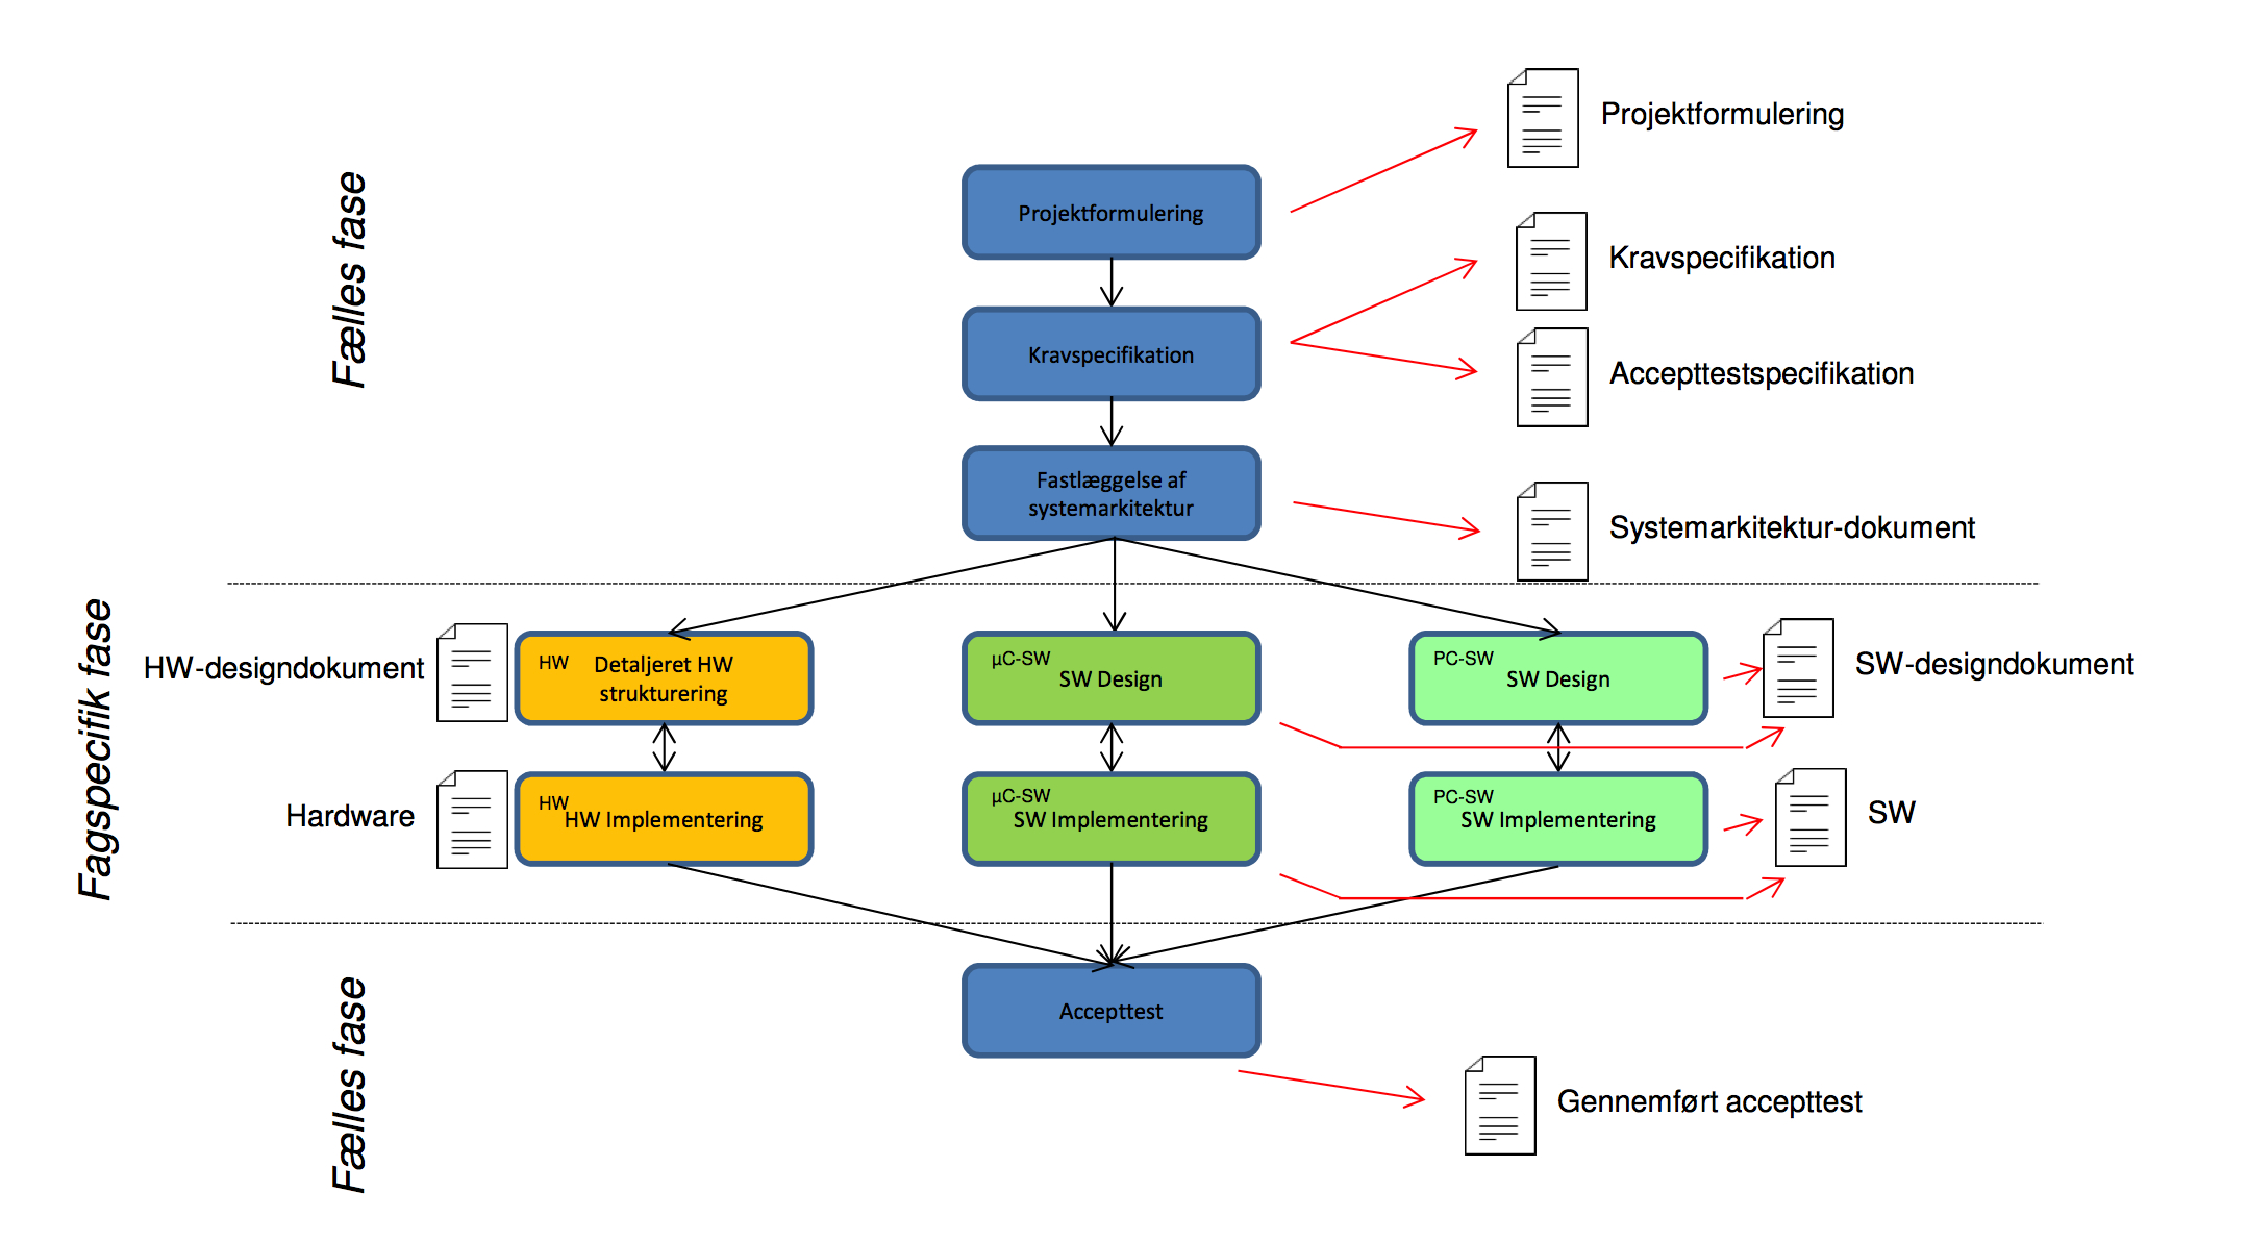
\includegraphics[width=\textwidth]{Billeder/ASE_modellen}
    \caption{ASE-modellen}
    \label{fig:ASE_modellen}
\end{figure}

V-modellen, se figur \ref{fig:V_modellen}, er benyttet sammen med ASE-modellen. V-modellen bygger på at hver enkelt del fase afsluttes før en ny del fase påbegyndes. En test af hver fase planlægges ved slutningen af hver fase. 

%V-MODELLEN BILLEDE
\begin{figure}[h]
  \centering
    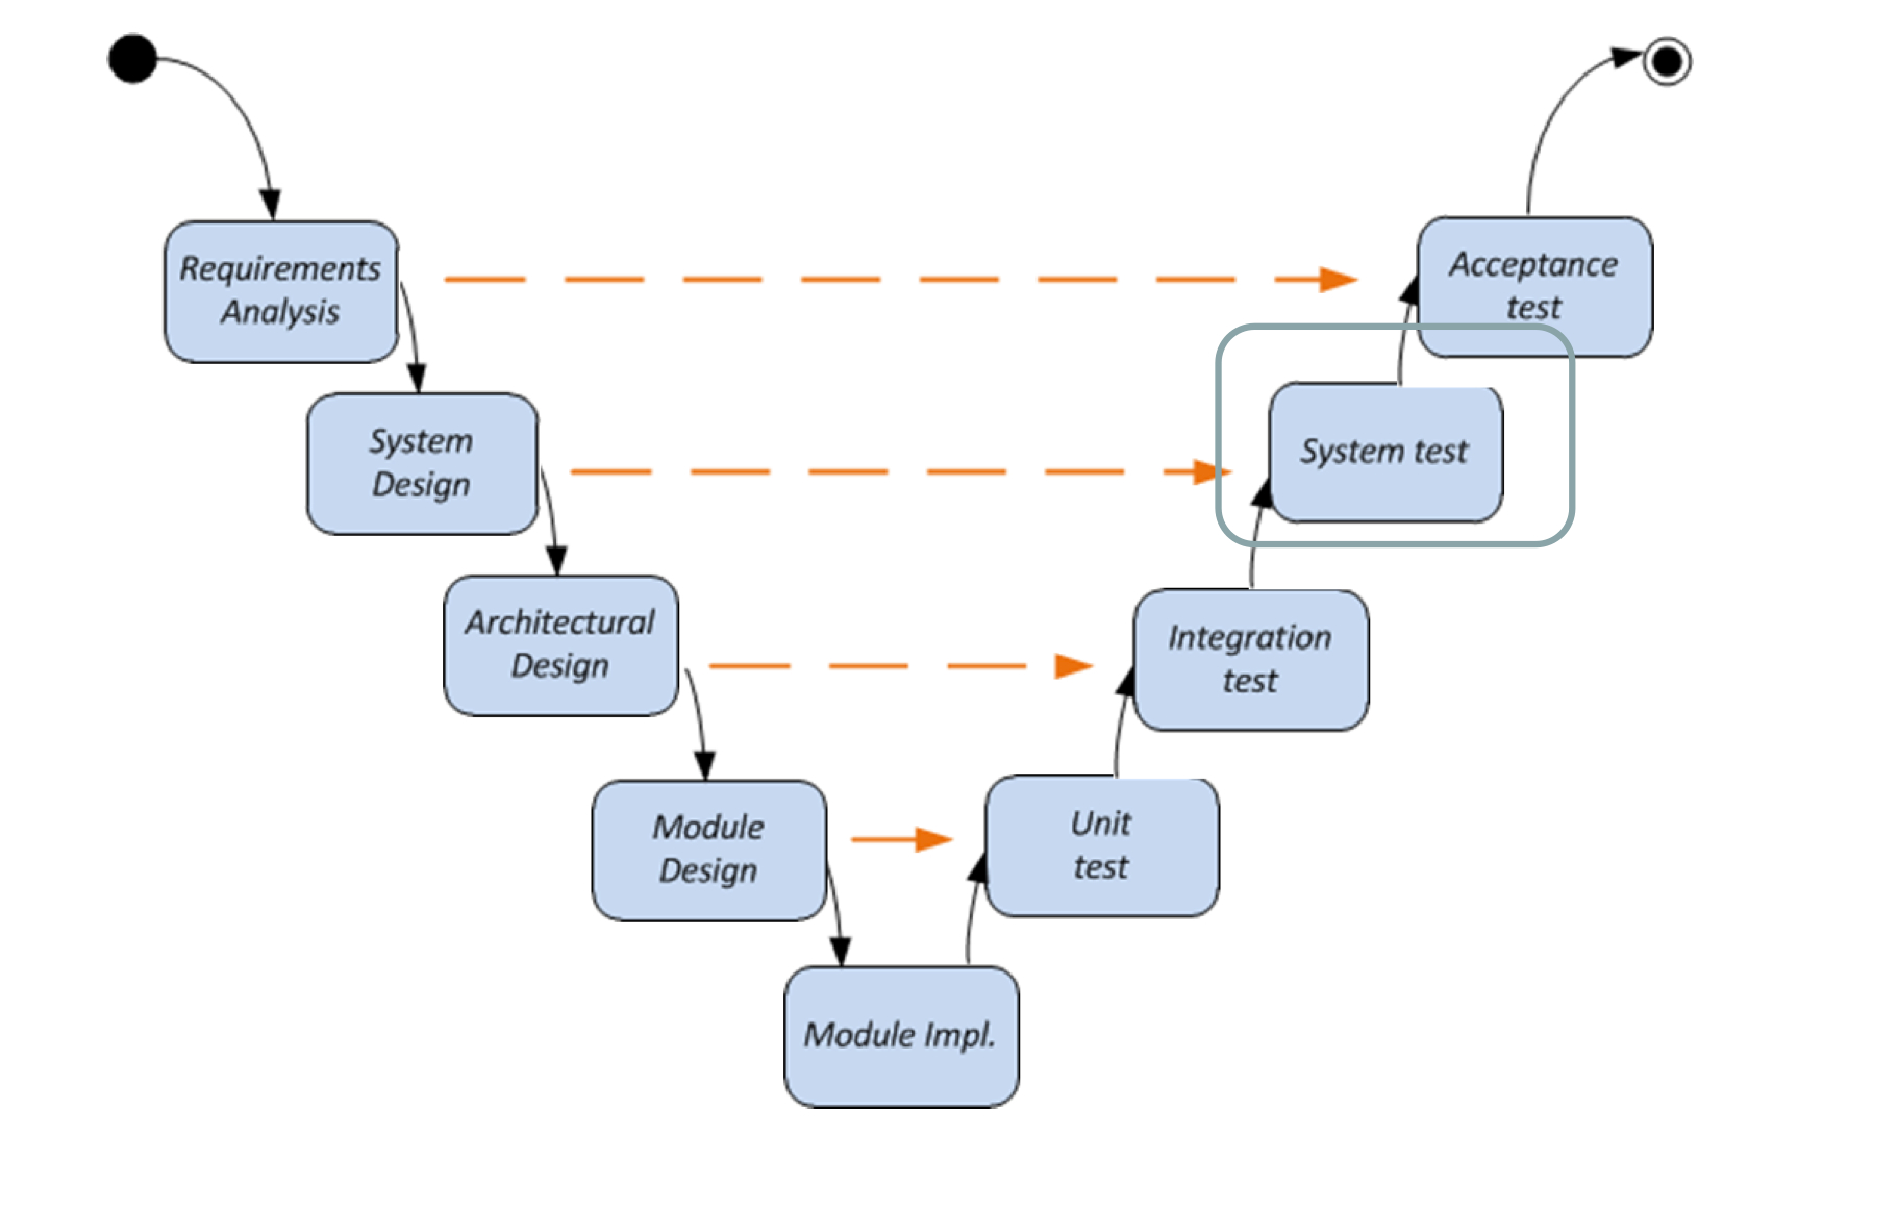
\includegraphics[width=\textwidth]{Billeder/V_modellen}
    \caption{V-modellen}
    \label{fig:V_modellen}
\end{figure}

\section{Møder, tidsplan, logbog og referater}

I forbindelse med gennemførelse af dette projekt er der afholdt en række møder. Gruppemøder, vejledermøder samt reviewmøder. 

Som hovedregel har der været afholdt et vejleder møde og mindst et gruppemøde hver uge, dog med enkelte undtagelser. 

Vejledermødet har været fast hver tirsdag. Dette møde har fungeret som den primære kontakt mellem gruppen og vejleder. Vejleren har ofte haft adgang til foreløbig dokumentation, som vejlederen har givet konstruktiv feedback på.

Gruppemøderne har haft et fast punkt: Status, hvem er i gang med hvad og hvor langt er hver i sær med de de pågældende opgaver? Ydermere er der afholdt 3 trivsels runder. Disse trivsels runder giver mulighed for at give ris/ros til de enkelte gruppemedlemmer og de giver mulighed for at gøre opmærksom på ikke projekt relaterede emner. 
Gruppen har fra start udarbejdet en gruppekontrakt\footnote{Gruppekontakten foreligger på bilags-CDen navn: Gruppekontrakt.pdf}, denne kontrakt udgør et fælles standpunkt for gruppen og de indbyrdes aftaler. Gruppen indførte et koncept kaldet ''Stå-op-møde'', dvs et møde der tager under 10 minutter, mødets mål er planlagt, således at tiden ikke spildes. 

Der er afholdt reviews. Ét review af kravspecifikationen samt et review af systemarkitekturen. 
Disse reviews har fået afklaret nogle problemstillinger som reviewgruppen fremlagde. 
Gruppen aftalte efter samtale med gruppe 2, at aflyse review af deres ststemarkitektur, da gruppe 2 ikke ville vente med at rette dokumentet til før review var modtaget.  

Alle møder er skrifteligt dokumenteret af sekretæren med både logbog og mødereferater. 

Tidsplanen\footnote{Tidsplanen forefindes på bilags-CDen. Navn: Tidsplan.pdf} er løbende blevet opdateret 

\section{Arbejdsfordeling}

Gruppen har som helhed haft et godt og solidt samarbejde. 

Allerede 1 måned efter projekts start oplevede gruppen ustabilitet i Jeppe Stærks fremmøde. Jeppe havde private problemer, som vi i gruppen selvfølgelig mente, at han skulle have tid til. Sidste gang vi så og hørte fra Jeppe var i uge 41. Siden har han af ukendte årsager valgt at ignore alt kontakt til gruppen og dens medlemmer. Gruppen valgte så d. 27/10 at meddele Jeppe skrifteligt, at han fra dags dato var ude af gruppen.     

\subsection{Arbejdsgrupper}
Gruppen har hovedsagligt været opdelt i 3 mindre arbejdsgrupper i forbindelse med faserne: Design, implementering og modultest. Forfattere til de enkelte kapitler er angivet med initialer.
Overordnet er opdelingen: HW (Jakob, Lennart, Mick, Poul og Simon) og SW (Bjørn og Jesper) 
HW og SW har arbejdet i nedenstående 3 undergrupper.

\textbf{Gruppen indeholdende Bjørn og Jesper} \newline
Bjørn og Jesper har stået for alt software over API niveau.

\textbf{Gruppen indeholdende Jakob og Lennart} \newline
Jakob og Lennart har primært arbejdet med FT-sensoren, både HW og SW mæssigt. Undervejs i forløbet er arbejdet delt lidt op, så Jakob hovedsageligt arbejdede med softwaren til PSoC4 og Lennart med den fysiske hardware. Der har været et godt arbejde og udregning af filteret samt designet af hele sensoren blev lavet sammen mens implementering heraf blev delt mere op. 


\textbf{Gruppen indeholdende Mick, Poul og Simon} \newline
Mick, Poul og Simon har igennem designfasen arbejdet tæt sammen om SPI kommunikationen, PIR-sensoren, Vandpumpe med tilhørende relæ og tilslutningsprintet. Mick og Poul har herfter stået for implementeringen af SPI kommunikationen, mens Simon har færdiggjort de andre dele samt implementeret tilslutningsprintet.


\subsection{Rollefordeling}

\textbf{Opsætning \LaTeX dokumenter} \newline
Hovedansvarlig: Mick 

\textbf{Sekretær i forbindelse med logbog og referater} \newline
Hovedansvarlig: Simon

\textbf{Projektleder, mødeindkalder og holder samt tavlestyring } \newline
Hovedansvarlig: Poul

\textbf{Vejlederkontakt} \newline
Hovedansvarlig: Poul   
